\documentclass{sig-alternate-10pt}
\usepackage{url}
\usepackage{framed}
\usepackage{amsmath}% http://ctan.org/pkg/amsmath
\usepackage[titlenumbered,ruled]{algorithm2e}
\usepackage{graphicx}
\usepackage{comment}
\usepackage{hyperref}
\usepackage{authblk}
\usepackage{soul}
\usepackage{color}
\usepackage{bbm}

\usepackage[font=footnotesize,labelfont=bf]{caption}
\usepackage[nameinlink]{cleveref}
\usepackage{xparse}% http://ctan.org/pkg/xparse
\NewDocumentCommand{\ceil}{s O{} m}{%
  \IfBooleanTF{#1} % starred
    {\left\lceil#3\right\rceil} % \ceil*[..]{..}
    {#2\lceil#3#2\rceil} % \ceil[..]{..}
}

\newcommand{\rks}[1]{\textcolor{magenta}{Rakesh: #1}}
\newcommand{\xin}[1]{\textcolor{red}{(XIN: #1)}}
\newcommand{\kelvin}[1]{\textcolor{blue}{(KELVIN: #1)}}
\newcommand{\Note}[1]{\textcolor{green}{(Note: #1)}}


\DeclareMathOperator*{\argmin}{arg\,min}
\DeclareMathOperator*{\argmax}{arg\,max}

\begin{document}

\title{OpenCell: Exposing Cellular Performance Metrics for DASH-based Video}
\author[1]{\large X. Kelvin Zou,\thanks{The work is done when Kelvin Zou is interning at AT\&T lab} }
\author[1]{\large Xin Jin}
\author[2]{\large Jeffrey Erman}
\author[2]{\large Vijay Gopalakrishnan}
\author[2]{\large Emir Halepovic}
\author[2]{\large Rittwik Jana}
\author[1]{\large Jennifer Rexford}
\author[2]{\large Rakesh K. Sinha}
\affil[1]{ Department of Computer Science, Princeton University, Princeton, NJ} \affil[2]{ AT\&T Labs -- Research, Bedminster, NJ}
\affil[1]{\texttt{\{xuanz, xinjin, jrex\}@cs.princeton.edu}} \affil[2]{\texttt{\{erman, gvijay, emir, rjana, sinha\}@research.att.com}}


\maketitle


%\begin{abstract}
%...
%\end{abstract}
\section{Introduction}
\label{sec:intro}

Video streaming has been a dominant application traffic in cellular networks, it consists
up to 40\% of the peak load~\cite{LTENetwork, VideoMeasureatt}. Although
the video streaming has become one huge part of cellular networks, most video streaming algorithms are designed only for wireline networks~\cite{BBA, QDASH, Festive}. Unique characteristics from the cellular networks, such as bandwidth un-predictability over short period of
time due to handoff or fading effects, create a challenge for a satisfactory
video streaming service. 

Most of the current video streaming services are using DASH (\textbf{D}ynamic
\textbf{A}daptation \textbf{S}treaming over \textbf{H}TTP)~\cite{DASH} based
end-to-end approaches. It uses chunk-based downloading and adjusts its video
streaming bit rate based on the play progress and the monitored bandwidth. The
application stitches video chunks together to provide a continuous playback.
However most of the video streaming service are not tailored for cellular networks, and they suffer from a conservative bandwidth estimation and video quality oscillation due to a lack of knowledge for the network condition. 
Some low layer connection information such as signal information is hard to access from application layer without root access.
End-to-end mechanisms~\cite{Sprout, QDASH, Festive} have been proposed to estimate link throughput, however some aims to reduce the packet delay while trading off the throughput, while others are making conservative and rough estimation. Periodical downloading behavior~\cite{OnOff} makes the bandwidth prediction even harder.
%For TCP throughput, the application need constantly saturate the link for a better estimation and the estimation takes a long time to converge, which can be hardly used in video streaming case where downloading is periodical\cite{OnOff,Sprout}. 
%\xin{Not sure if this is correct. Can they be collected from end
%hosts? Cite some papers or explain why it's hard}, \kelvin{ how does this sound like now?}

On the other hand, a cellular network service provider has much better knowledge of the connection
conditions for the clients via monitoring, as the last mile has long been identified as the
bottleneck\cite{LASTMILE}. Cellular ISPs also know the number of
active users in each cell and proportional fair packet scheduling system, and thus can make more
precise predictions in terms of available bandwidth. In fact, many key statistics like radio information and the base station utilization can be easily and some are
already being collected within carriers. 

Given cellular carrier's advantages, there are some proposals\cite{Avis} for an in-network video streaming framework where the network controls video streaming algorithm. 
Nevertheless it also suffers from some limitations. First it
lacks the application knowledge such as client video buffer occupancy and may lead to re-buffering. 
Second different users may apply different subscription
policies w.r.t.video quality (Spotify already has low quality and high quality for free and premium users, video service may apply the same concept) and streaming service providers may
hesitate to share user information with ISPs. Users may also have data budget concerns. Last
but not least, in-network approaches may require the modification of packet scheduling system and this
is hard in practice as most carriers are using pre-installed
vendor-specific scheduler. 

To address the issue, we propose a joint optimization between the cellular network (ISP) and video streaming service (CP): ISP exposes its estimated bandwidth to CP, and CP adjusts its streaming service decision based on the estimated bandwidth. By doing so video streaming service can achieve higher quality and reduce the amount of chunk prefetching, and thus save data budget and power consumption. ISPs also benefit from less bursty traffic and avoid excessive queueing delay from flow pacing. There are three main contributions in this paper:
\begin{itemize}
\item Design a scalable architecture to compute  and expose them to video streaming providers on the fly.
\item Conduct a measurement study to show the predictability of user channel quality and cell loads. 
\item Design an algorithm to show that by using the KPIs we have a significant improvement in video streaming service.
\end{itemize}

This paper introduces a scalable architecture to compute the bandwidth and expose the KPIs to the service provider in \autoref{sec:Architecture} and then we conduct a preliminary measurement study of predictability of available bandwidth in \autoref{sec:prediction}. We propose our new optimization algorithm in \autoref{sec:optimization} and show our results in \autoref{sec:evaluation}. This paper concludes in \autoref{sec:conclusion}. 


=============== [rjana,gvijay] 

Increasing number of users are watching videos on their cellular
devices. Recent studies~\cite{cisco-vni} show that mobile video
accounts more than 50\% of the cellular traffic today and is expected
to grow fourteen fold by 2018. This growing popularity of video over
cellular networks has attracted significant attention with cellular
operators making huge investments to provide better coverage and
capacity, content providers adopting state-of-the-art delivery
mechanisms a like Dynamic Adaptation Streaming over HTTP
(DASH)~\cite{DASH} and HTTP Live Streaming (HLS)~\cite{HLS} and
researchers proposing mechanisms~\cite{HLS,Festive,BBA} that optimize
on metrics such as average video quality, number of interruptions, or
the stability of video quality.

Despite these novel delivery mechanisms and expensive network
investments, the quality of experience for users watching videos over
cellular networks remains low. A recent study~\cite{opera-stall} shows
that between 40\% and 73\% of all videos played on mobile networks
experience stalls. For every 60 seconds of video, users on 3G
experienced an average of 47 seconds of stall, while those on LTE
experienced 15 seconds stall~\cite{citrix-stall}. Worse yet, the
fraction of videos stalled increased with video quality with 10.5\% of
240p videos stalling while 45.7\% of 720p videos experienced a
stall. 

We believe that one of the main reasons for the low quality of
experience is the mis-match between information used by video
adaptation process and available network bandwidth. The adaptation
process on a video client has to decide on the video quality for each
chunk. To do so, it uses historical throughput as an estimate of the
client's current bandwidth. Based on its estimate of available
bandwidth, the client picks a certain video quality for the chunk. On
cellular networks, however, this estimate could be widely off. There
are many factors, including the user's signal strength, number of
users in the cell, the congestion in the cell, and user mobility that
can determine a user's bandwidth. As a result, a user's bandwidth can
vary widely even over short periods of time, rendering any historical
estimates inaccurate. Consequently, as we show in
Sec.~\ref{sec:background}, the client ends up either under- or
over-estimating its available bandwidth.

Our approach to tackling this issue is to move the task of bandwidth
estimation from the client to the cellular network. We envision
opening up the cellular network (e.g., through an API) to provide
hints to a client's player about the bandwidth available to that
client for a future time duration (typically few seconds). Our
motivation stems from the fact that the cellular operator has a global
view of all traffic that is flowing through their network. This
includes information such as users' signal strength (RSRP), wireless
channel quality (CQI, RSRQ), the number of users, users' mobility
patterns, etc. Further, the operator knows how the different
middleboxes in their network will affect this user's flow and know of
different priority treatments applicable to this user's
traffic. Having visibility of all competing flows inside the network
allows the cellular operator to {\em predict} every user's bandwidth
for a future time period. For example, the operator can predict, using
all this information, how a scheduler operating inside a base station
would rank the user and how much cellular resources it would allocate
for that user. This directly translates to the bandwidth that a user
would get.

In this paper, we first show that existing methods used by clients to
estimate cellular network bandwidth are indeed deficient. Then we
study if video quality of experience improves if we have accurate
network bandwidths. To do so, we use an oracle in an off-line mode to
provide predicted throughput. We show, using this oracle, that there
are significant improvements to be had by having accurate network
bandwidth information. This result also serves as an upper-bound on
the possible improvements. Next, assume that network information is
available to us, we show how we can predict the available bandwidth in
an online manner. Since existing video client algorithms are not aware
of our predictions, we design a client algorithm that uses this
information and compare its performance to the state-of-the-art
approaches (i.e., FESTIVE~\cite{Festive} and BBA~\cite{BBA}). Our
results show that our algorithm performs better than both these
approaches. Finally, we propose various mechanisms through which our
predicted bandwidth can be made available to video clients.


\section{Measurement study}\label{sec:prediction}
In this section we conduct an extensive measurement study to show the predictability of a few key metrics that affects the available throughput. 

Proportional fair schedulers have been widely deployed in 3G and 4G networks to achieve high spectrum efficiency. It takes the channel conditions and the number of active users as inputs and schedules packets accordingly. In this section, we study how accurate prediction can give us for the two key inputs-channel condition and the number of active users. The information can be mapped to an available throughput, however we have not fully explored the underline relation between them. This approach is different from end-to-end monitoring approaches as it does not require constantly saturating the link to get the maximum bandwidth. 

The traces are collected for 5 minutes in Jun 2014 over several geolocations in the United States from one major 4G network carrier, it covers more than half million users and over 2000 eNodeBs. The traces have been anonymized before handing to us for privacy reasons. 

\begin{comment}
\subsection{Proportional Fair Scheduler}\label{subsec:ltenet}
3G ad 4G networks are using Orthogonal Frequency-Division Multiuser Access(OFDMA) scheme to achieve high spectrum efficiency. To achieve multiuser diversity, NodeBs and eNodeBs are running variations of proportional fair scheduling system. A basic \textit{proportional fair scheduler} works as the following: eNodeBs obtain the feedback from each user about their instantaneous channel quality conditions (CQ) in terms of encoding rate per resource block, and take the ratio between it and historical mean of CQ and pick the user with the maximum ratio. In a static model over a long term, each user will get 1/N share of resource blocks if N is the static number of users in the cell, a dynamic model also has a similar result\cite{PFINFOCOM}. The maximum bandwidth for each user in a cell is a function of: $T$-number of resource blocks in the cell, $N$-number of users in the cell, and $\mathbf{CQ}$-channel quality vector for all users; so maximum bandwidth vector for all users $\mathbf{BW} = f(T, N, \mathbf{CQ})$. We do not directly address $f(T, N, \mathbf{CQ})$ function in this paper as it is a vendor-specific PF-based scheduler. In the rest of the paper we assume a simple PF scheduler model, that is $\mathbf{BW} = f(T, N, \mathbf{CQ})=\frac{T}{N}*\mathbf{CQ}$. Among the three variables, $T$ is predetermined by the hardware, $N$ and $\mathbf{CQ}$ are the two factors we need to predict. 
\end{comment}

%\subsection{Bandwidth Estimation} \label{subsec:Prediction}


\subsection{Predictability}
There are many different metrics to compute the accuracy of a prediction, such as Mean Absolute Percentage Error (MAPE), Mean Square Percentage Error (MSE). In this paper we use MAPE since it can give us a good hint about how much off the prediction is from the true value for each step. In addition, we have the analysis of Cumulative Forecast Error (CFE), as it indicates how biased the prediction is over a long term. 

\begin{figure}[t]

\begin{minipage} {\linewidth}
\centering
 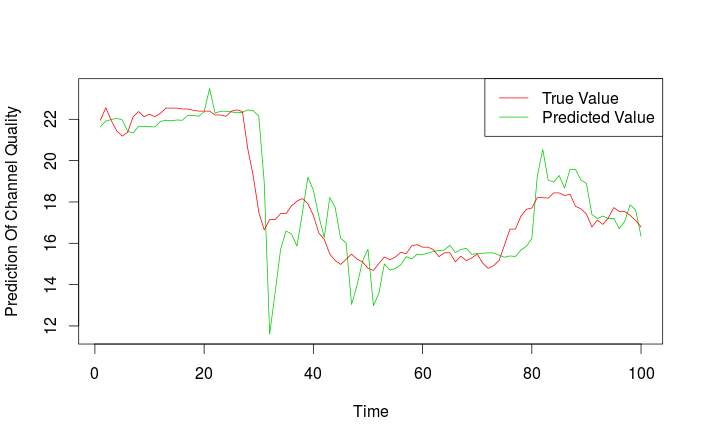
\includegraphics[width=\linewidth]{pictures/prediction.png}
\end{minipage}
\hspace{0.5cm}
\begin{minipage} {\linewidth}
\centering
 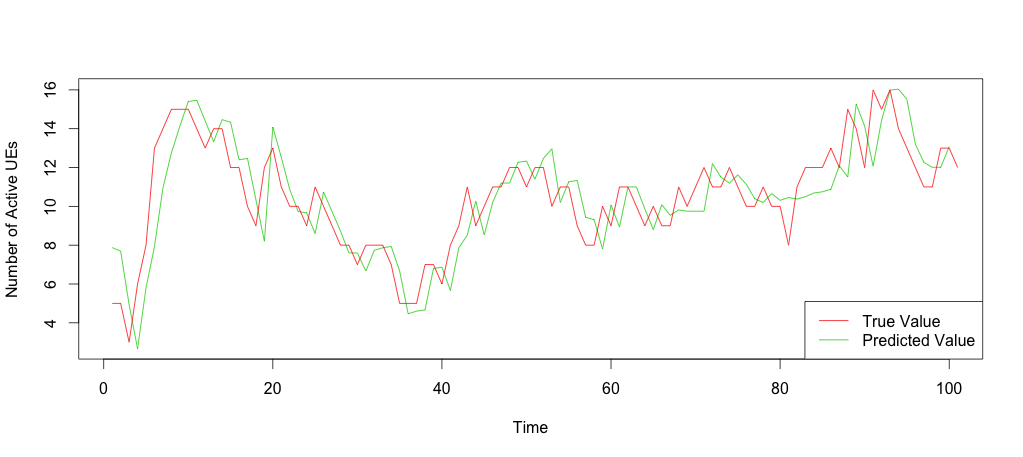
\includegraphics[width=\linewidth]{pictures/UE.png}
\end{minipage}

\caption{prediction for channel quality and active UE} \label{fig:prediction}
\end{figure}

\subsection{Channel Quality}\label{subsec:CQ}
One unique characteristic for cellular network is the high mobility and this causes the link quality to fluctuate to a certain extent.

\emph{RSRQ:} Reference Signal Received Quality, is the key metric for the LTE wireless channel. RSRQ senses the load from other users in the same cell and the neighboring cells, and is indexed in 0-34 integer numbers; a higher number indicates a better link quality. RSRQ values can be mapped to certain encoding rate.

We predict the future RSRQ using time series analysis, in particular we use ARIMA (Auto-Regressive Integrated Moving Average) model to predict the next second: the algorithm fits the best ARIMA with historical data, and it uses a sliding window as the training dataset. We set window size to 15s. (We tried longer window but see no significant improvement over accuracy.) 

Through replaying 113 sample traces where the UEs are active for more than 100 seconds, we found that MAPE$<0.18$ for all the users, and the mean value is $0.064$. CFE values varies more across users with a maximum CFE=34.6, this is about three times of a unit value. In other words, for a 100 seconds prediction, prediction result may be 97\% accurate over long term and 82\% accurate on average for each prediction. 

The above results tell us that a simple prediction model such as ARIMA can offer a fairly accurate prediction. 

\subsection{Cell Load}\label{subsec:NUser}
We measured the number of active users in each cell from the same trace as mentioned above. The trace is collected from UE's RSRQ reports to eNodeBs. We assume a user is active in a certain second if the user reports RSRQ in a one-second interval. 

We apply ARIMA model, and find in most cases a random-walk model fits in the best. Different cells have different load, and the prediction works better in a heavily loaded cell. Since the inverse value of the active user number has a strong correlation with available bandwidth for each user, we take the inverse value to compute MAPE. For heavily loaded cell ($>30$ UEs) we have MAPE$<0.1$, and medium loaded cell (5-30 UEs) MAPE$<0.3$. This tells us we can achieve 70\% accuracy for each prediction on average for a medium to heavily loaded cell. For a lightly loaded cell, the prediction is not very satisfying, with MAPE$>1$. This is because the prediction value are affected to a greater extent by the small true value. However for a lightly loaded cell each user usually has higher available bandwidth, and thus has less need for extra information such as bandwidth informing.  

\begin{comment}

\section{Design} \label{sec:optimization}
In this section, we explain the reason to choose an \textbf{\emph{end-to-end decision making with in-network knowledge}} model in section \ref{designchoice}, we then explain the our architecture in section \ref{architecture}. 
%introduce performance metrics in section \ref{metrics} and 

\subsection{Who decides the video streaming?}\label{designchoice}
For video streaming service decision making, there are three different models: \emph{In-network}, \emph{strictly end-to-end} and \emph{End-to-end with in-network knowledge}. 

\emph{In-network techniques} make decisions for users: it selects the video bit rate and schedule the download for users based on its knowledge of the network condition. However in-network approaches lack the insight of the video play progress, e.g., video buffer occupancy since it does not deal with any video decoding. Aside from technical reasons, here are several privacy/policy reasons for not doing this: most content providers are using encrypted http connections which ISPs cannot access; users may be concerned about their data budgets and thus not choose high bit rate; or content providers have different video play bit rate policies for different users based on their subscription contracts. 

\emph{End-to-end techniques} probe the network condition based on round trip time (RTT) and historical throughput, however existence of the proxy makes the RTT very inaccurate as it splits tcp connections. The dynamic nature of the wireless link makes historical data unable to capture the link behavior, e.g. the available bandwidth may plummet due to fading effects or handoff and recovers very soon after, current end-to-end approaches fail to react to those scenarios in most cases.

\emph{End-to-end with in-network knowledge} model addresses the above issues: instead of making the decision for the client; the network helps video streaming service make better decisions via offering some key performance metrics about the network condition, such as available throughput and handoff. 

Though an end-to-end with in-network knowledge approach has advantages over the other two, we still need to address the problem of how to expose the in-network knowledge in a least intrusive way in a scalable manner. 







\subsection{Architecture}\label{architecture}

We propose a two-tiered system for to implement OpenCell system. The two parts sit in RAN and EPC respectively. 

At the lower tier we have bandwidth estimator for each eNodeB. Estimating link channel quality and cell load is much more scalable if if we compute it at eNodeBs, since there are only hundreds of users at each cell, while aggregated number of users for a SGW can be tens of thousands. Making an estimation at second level means for each user the computational cycle is ~1 $ms$ if sitting at eNodeBs and ~10  $\mu s$ if sitting at Serving Gateway. Processing the raw information such as RSRQ from eNodeBs and extract it as estimated bandwidth also reduces the extra traffic generated for message passing. 

At the higher tier, the information inferred at eNodeBs are received at the proxy, and combined with handoff information, we make a final estimation of available bandwidth for each user and then expose this piece of information to application service providers by some means. The architecture is in figure \ref{cellular}.

\begin{figure}[t]\label{cellular}
\begin{minipage}[b]{\linewidth}
\centering
 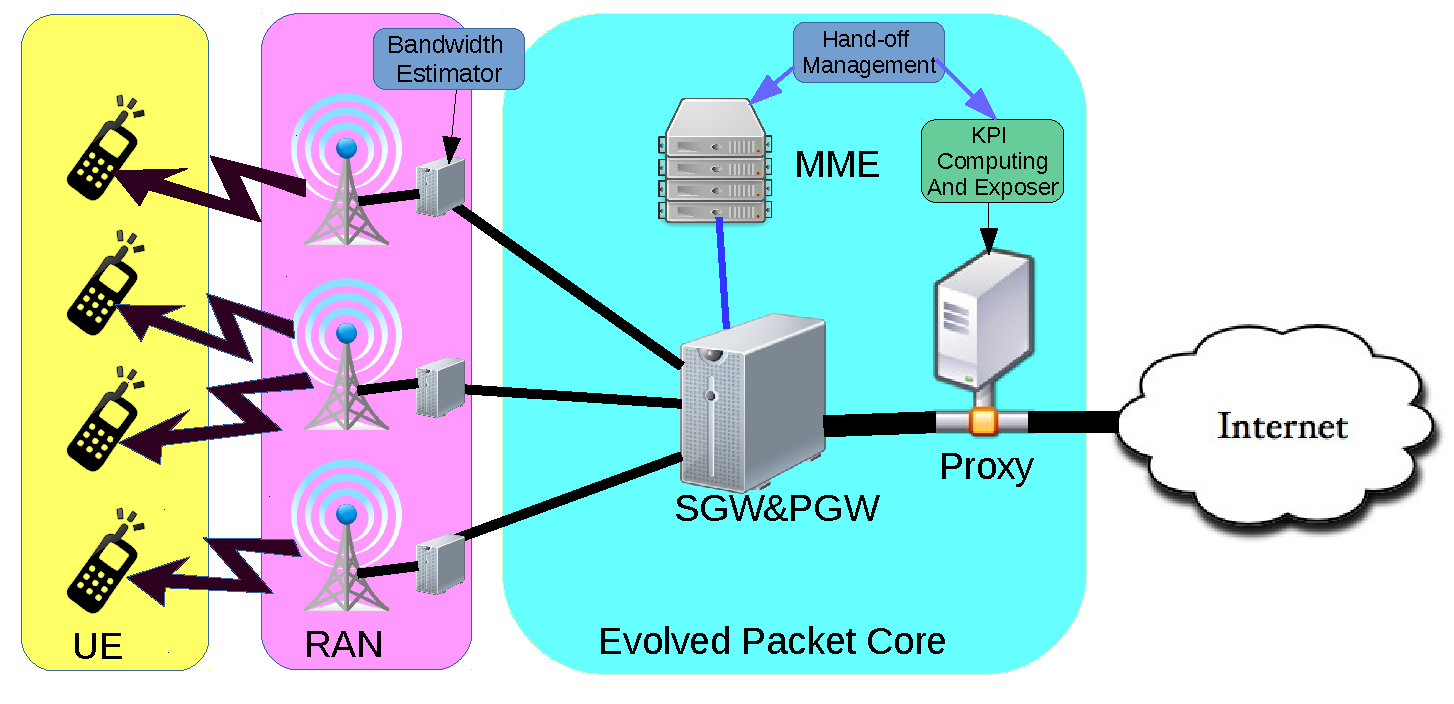
\includegraphics[width=\linewidth]{cellular.pdf}
\end{minipage}
\caption{OpenCell Design}
\end{figure}

In terms of how to expose the API information, there are three options: encapsulation (i) at TCP/IP layer, (ii) at application layer; and (iii) using a distinct channel. Each approach has its pros and cons, for example TCP/IP layer does not require DPI but the fields used for encapsulation might be overwritten deep in the network from middleboxes. Using distinct channel does not suffer either problem but it requires application service providers' cooperation. We are still weighing between the options and leave this as a future problem. 



\end{comment}

\section{Video Streaming optimization}\label{sec:optimization}

We design a video rate selection algorithm to exploit reliable
prediction of available future bandwidth.

% The impact of reliable prediction of available bandwidth , how this
% can be reflected in the improvement of video streaming service has not
% been explored. In this section we show that the algorithm can use the
% available bandwidth as a key information and make a smart decision.  

We start by defining performance metrics for video streaming service in
\autoref{subsec:metrics}. The goal of the video rate selection is to 
optimize these metrics.
% takes the metrics into consideration during video quality selection. 
In \autoref{subsec:offline}, we design an optimal offline algorithm
that takes available bandwidth during the entire session as input and
selects video quality for each chunk. We assume constant bit
rate encoding, meaning that all chunks for a given video rate have the
same size.
% For a certain video play bit rate, we assume the encoding rate is constant.

  
The performance of this algorithm forms an upper bound on possible
gains from knowledge of future bandwidth.
In \autoref{subsec:online}, we present our final algorithm that, for
each chunk, first selects a reference video rate  based on prediction of 
available bandwidth in the \emph{near} future. 
Then we further refine this rate selection based on buffer occupancy
(current value as well as change in last few chunks).
%
%This algorithm uses the predicted bandwidth 
%for the next video chunk interval to compute a reference play bit
%rate, and uses this referred bandwidth,  
%play history and buffer occupancy to make a final decision. 
\rks{It is not very clear if we are (a) designing a video rate
  selection algorithm that is simply better than BBA, FESTIVE,
  etc. while using the similar information as those guys,
  or (b) custom designing an algorithm to exploit knowledge of future
  bandwidth? If it is the latter, it needs to be pointed in the
  text. E.g., we can afford to be more aggressive because we have
  higher confidence in our bw estimate. If it is the former, it is a
  very strong claim that needs more validation.}

\kelvin{To answer your question, I think this might be  both, FESTIVE also uses estimated bandwidth in a conservative manner, so their stability adjustment is simpler. I tried to use
FESTIVE with prediction, but it cannot just fit in seamlessly}

\subsection{Performance Metrics}\label{subsec:metrics}

We quantify the performance of our algorithm with the following three
metrics, which have been extensively used in prior research work in video
streaming 
\cite{Qava, Avis,VideoMeasurement, Festive}. 

% To help us understand what extra benefit we can achieve from new
% information, we define \emph{three} performance metrics for video
% streaming. These metrics have been extensively studies in various
% video streaming algorithms and we use the metrics in both design and
% evaluation\cite{Qava, Avis,VideoMeasurement, Festive}. 

\begin{enumerate}
\item\textit{Quality}: as the video download is chunk-based, a video
  session can consist of chunks with different qualities (bit
  rates). The video player should download the chunk with the highest
  possible quality based on available bandwidth at each download point
  to give user better quality experience. We define quality as 
  $E = \frac{\mbox{total size of played video}}{\mbox{sum of available bandwidths}}$.
% \xin{Maybe use formula? It looks a bit awkward now.}

\item\textit{Stability}: From viewer's perspective, frequent rate
  switches are distracting and undesirable. Our goal is to minimize 
  % To assess the stability of video streaming, we  define
  \emph{instability}, defined as the number of rate switches.
% between consecutive chunks (\rks{rate switch, by defn, is between
% consecutive chunks, right?} so I commented it out but I don't feel
% strongly about it so you are welcome to put it back.
% \phi= \sum\limits_t
%  \mathbf{1}(R^t!=R^{t-1})$, where $\mathbf{1}$ is an indicator
%  function. 
% From Rakesh: I commented out this part as we have not defined R^t
% and I thought that most readers will understand what we mean w/o aid
% of a formula. 
  
\item\textit{Interruption and rebuffering}: Video play should not be
  halted for rebuffering video chunks, otherwise user experience will
  be severely degraded. Video play interruptions affect the user
  engagement and results in early abandonment of the video play
  ~\cite{VideoMeasurement}. We minimize the 
  number of interruptions over the entire session. % whole play time. 
\end{enumerate}

\begin{table} [bt]
\small
\begin{tabular} {|c |l |}
\hline
\textbf{Symbol}&\multicolumn{1}{c|}{\textbf{Meaning} }\\ \hline
$T$ &number of video chunks  \\ \hline
$CD$ & chunk duration  \\ \hline
$M$ &number of video quality levels (encoding bit rates)\\ \hline
$R_i$& rate for the video with $i^{th}$ highest encoding bit rate \\ \hline
$x_i^t$& binary variable indicating whether $R_i$ is the video \\
& play rate at time $t$ \\ \hline
% indicator of encoding of $R_i$ video play rate at time t
$E$& bandwidth utilization $= \frac{\mbox{total size of played
    video}}{\mbox{sum of available bandwidths}}$ \\ \hline
%of video download over available bandwidth 
$\phi$ &number of video rate switches \\ \hline
% for a video play
$C $ & predicted bandwidth for the next chunk\\ \hline
$B_t $ & buffer occupancy (seconds of video) at the time \\
     & of download of $t$-th chunk \\ \hline
$z $ &maximum buffer size (seconds of video) \\ \hline
$B_{risk} $ & threshold for buffer occupancy. Below this threshold is\\
& \emph{risky} zone; above this threshold is \emph{safe} zone \\ \hline
\end{tabular}
\centering
\caption{Variables and parameters for optimization}
\label{tab:notation}
\end{table}
\subsection{Video Quality Upper Bound}\label{subsec:offline}


Given the available bandwidth for the \emph{entire} video play
session, we want to know the optimal video rates for each chunk. This
is an idealization of our real problem, where we only know (with high
confidence) available bandwidth for a few chunks.
We formulate a Mixed Integer Linear Program (MILP) with the goal of
maximizing quality without causing any interruptions. To keep this
presentation simple, we only focus on quality here and ignore stability. 
\rks{A possible criticism we may face is that, based on MILP, we may
  claim that there is room for say 30\% improvement but reader may
  counter that if we also cared for stability, the gap may only be 
  10\%. Can we somehow say that ignoring stability does not change the
  results very much? May not be needed for workshop paper but for the
  longer paper.}

% quantify video quality (play efficiency)
% upper bound, e.g., 
% and play to best
% utilize the available bandwidth. We prioritize interruption-free and
% allow prefetching unlimited video chunks.  

Table~\ref{tab:notation} lists the variables and parameters.
In reality, we need chunks ahead of their actual playing
time. E.g., we need one chunk before we can start the video. To keep
this formulation simple, we ignore this restriction here.

To ensure  no interruptions, at each chunk, the total download
should not exceed the sum of capacities until that video chunk.
% always be at least be equal to video played 

% For simplicity, we assume that at the initial
% state,  
% the client video buffer contains one chunk ahead of playing.
% ), i.e.,


%The download rate at chunk $t$ is given by the rate selected at that chunk. 
Because for any $t$, exactly one $x_i^t$ is one, the video play rate 
% download rate: Rakesh the download and play times are shifted so
% what we mean here is play rate and not download rate.
at chunk $t$ is given by 
$PlayRate(t) = \sum \limits_{i=1}^M R_i *  x_i^t$. 
The zero-interruptions constraint is 
%$\sum \limits_{t=1}^\tau  (\sum \limits_{i=1}^M R_i *  x_i^t)
%\leq\sum\limits_{t=1}^\tau C^t$
$\sum \limits_{t=1}^\tau  PlayRate(t) \leq\sum\limits_{t=1}^\tau C^t$
for $\forall \tau \in \{1, \dots, T\}$.
As stated earlier, quality (play efficiency) 
%at the end of a video session, the play efficiency 
is the overall utilization of the available bandwidth
over time period $[1:T]$, defined as
$E =\frac{\sum\limits_{t=1}^T  PlayRate(t)}{\sum\limits_{t=1}^T C^t}$. 
The MILP for maximizing quality without causing interruptions is
\begin{subequations}
\begin{align*}
&\textsc{maximize }&{E}\\ 
&\textsc{Subject to}\\
%&\sum \limits_{t=1}^\tau  \sum \limits_{i=1}^M R_i \cdot
%x_i^t\leq\sum\limits_{t=1}^\tau C^t& \forall \tau \in \{1, \dots,
%T\}\\
&\forall \tau \in \{1, \dots, T\}, \sum \limits_{t=1}^\tau  PlayRate(t)
\leq\sum\limits_{t=1}^\tau C^t \\
& \forall t, \sum \limits_{i=1}^M x_i^t =1\ \\
& \forall t, i, x_i^t = \{0,1\}
\end{align*}
\end{subequations}

\subsection{Video Streaming Algorithm} \label{subsec:online}

In the algorithm, we assume that the available bandwidth forecast for
a small time interval is known.
(In the evaluations, we are assuming that we know the bandwidth for
the next chunk.)
% in this paper we assume bandwidth estimation for one video chunk. 
The algorithm is a joint optimization
solution based on both the video buffer occupancy and the predicted bandwidth. 


We motivate our algorithm with a naive solution: pick the maximum
 play bit rate that can be supported by the known future bandwidth. 
There are several shortcomings: (i) the stability may be heavily
impacted due to highly variable bandwidth values, and (ii)
%interruptions may occur 
because we are using all of the bandwidth for maximizing quality of
the video, there is a good chance that our playout buffer will not
have many chunks. 
Connection loss (zero or near zero bandwidth) of several seconds is
not uncommon in  cellular networks and these may drain out the buffer
and result in video interruption and rebuffering.
% It is not uncommon in cellular networks to 
%  and video will have interruptions if we face
% a few or even tens of seconds

% network. 
To avoid this, we divide the
buffer into two zones -- \emph{risky} and \emph{safe} -- based on
buffer occupancy 
threshold $B_{risk} $. 
We start with a reference video rate, $R_{ref}$, that we refine
further based on recent change in buffer occupancy.
In risky zone, buffer occupancy is smaller than
$B_{risk}$ and thus there is a
a high chance of buffer over-drain. So we try to build the buffer by
choosing $R_{ref}$ one rate lower than what the available bandwidth
can support. 
E.g., if the bandwidth is $0.58$ Mbps and two closest video
bit rates are $0.56$ and $0.375$, we choose $R_{ref}$ to be $ 0.375$
Mbps in the risky zone. 
The idea, as stated earlier, is to quickly 
fill in the client buffer to a safe level.
In the safe zone,  $R_{ref}$ is the highest available bit rate, which
is $0.56$ Mbps in our 
example. 
% We call this computed bit rate reference bit rate, $R_{ref}$.
%  Choosing referred bandwidth would give us high play efficiency.  

\begin{algorithm} [t]
\SetAlgoLined
 \SetKwInOut{Input}{Input}
 \Input{ $C$: Predicted available bandwidth \newline
   $\mathbf{B}$: Buffer occupancy vector for last $k$ chunks
   \newline$R_{cur}$: Current video bit rate}
 \SetKwInOut{Output}{Output}
 \Output{$Rate$: Rate for next chunk. }
%pick MAX($R_{ref}$) where $R_{ref}<C$\;
\uIf{$B_t>z$}{
 Sleep for $B_t -z$ seconds\
 \
}
${ref} = \max \{i: R_i \le C\}$\;
 \uIf{$B_t\leq B_{risk} $}{
 $ref = ref-1$\;
 }
 \uIf{$R_{ref}<R_{cur}$ and $B_t \ge B_{risk}$ }
 {
   Rate=$R_{curr}$
 }
 \uElseIf{$R_{ref}<R_{cur}$ and $B_t<B_{risk}$ }
 {
 $\Delta B = B_{t} -B_{t-k}$\;
  \rks{if $\Delta B \le 0$ then rate = $R_{ref}$ and do not execute the next chunk, right?} \;
 \For{ $R\in [R_{ref}, R_{cur}]$}
 {
 $BufferLoss=CD*\frac{R-C}{C}$\;

 \uIf{$\Delta B>BLoss$}
 {Rate=$R$}
 }
 }
 \Else{
 \uIf{$R_{ref}>R_{cur}$} {
 \For{$R\in [R_{cur}, R_{ref}]$}{
 $BufferLoss=\alpha * (B-z) *\frac{R-R_{cur}}{R_{cur}}$\;
\rks{this expression seems incorrect. For one thing, $B-z < 0$. Pl. see my comment in the text}\;
  $\Delta B = B_{t} -B_{t-k} $\;
 \uIf{$\Delta B>BufferLoss$}
 {Rate=$R$}
 }
 }
 }
\caption{Rate Selection} \label{cap:algorithm}
\end{algorithm} 
Algorithm~\ref{cap:algorithm} gives the pseudo-code. 
The algorithm 
% considers the stability in the following manner: it
compares the reference bit rate, $R_{ref}$, and the current play rate,
$R_{curr}$. There are three possibilities which we examine in turn.
If $R_{ref}= R_{cur}$ then we have a simple decision; we pick the
video rate to be $ R_{cur}$.
If $R_{ref} \neq R_{cur}$, we need to balance the three somewhat
incongruent goals of stability
(as much as possible keep the rate at $R_{curr}$), zero-interruptions
(maintain buffer occupancy at a safe level), and high quality (pick
higher rates whenever possible). 
We use delayed updates \rks{elaborate what this means} 
based on the buffer occupancy status and ideas similar to what
was proposed in BBA \cite{BBA} and FESTIVE \cite{Festive} algorithms. 
At the high level, if $R_{ref} \le R_{cur}$, the algorithm still
stays at $R_{cur}$ if buffer occupancy is high (low chance of
over-drain) or if buffer gained significantly during the last few
chunks (can afford a little buffer loss this chunk). 
Similarly if $R_{ref} \ge R_{cur}$, we go to a rate higher than
$R_curr$ only if we estimate that we can sustain the higher rate for
next several chunks (e.g., higher buffer occupancy implies a greater
tolerance for buffer loss so we can pick a high rate).
\rks{Kelvin, pl. check that I captured the right intuition.}
We now state the precise logic of the rate selection algorithm.
% want to maintain the rate at 
% chooses the reference or current bandwidth or a play bit rate
% between them based on  certain criteria. It uses delayed updates
% based on the buffer occupancy status and uses ideas similar to what
% was proposed in BBA \cite{BBA} and FESTIVE \cite{Festive} algorithms. 
% At the high level, the algorithm tries to stay at $R_{cur}$, 
% unless either the bandwidth and recent buffer gains cannot sustain 
% that play bit rate so the algorithm jumps down to lower quality, 
% or the near future bandwidth is higher and recent buffer gains can sustain a 
% potential buffer loss if the bandwidth returns to a current bandwidth
% in a far future so the algorithm jumps up to higher quality.
% There are three possibilities w.r.t. $R_{ref}$ and $R_{cur}$, which we
% examine in turn.



If $R_{ref}= R_{cur}$ then we have a simple decision; we pick the
video rate to be $ R_{cur}$.
select rate as 

If $R_{ref} < R_{cur}$ then the current play bit rate is higher than
available bandwidth, the 
algorithm may choose current play bit rate at the cost of draining
client video buffer. If the buffer size is in safe zone, the
algorithm simply takes the risk and adheres to current play bit rate. If the
buffer is in risky zone, it computes the possible buffer drain if
choosing the current play bit rate $BufferLoss
=CD*\frac{R_{cur}-C}{C}$, because it takes $\frac{CD*R_{cur}}{C}$ to finish downloading 
$CD$ seconds of video. 
%\rks{please explain this formula. Is BW same as C?}
We compare the buffer change in
the last $k$ chunks where $k$ is a tunable parameter ($k=5$ in evaluation), 
% \rks{$k$ another parameter? Should we include in the table?}
$\Delta B = B_{t} -B_{t-k} + CD*k$, where $B_{t}$
represents the buffer occupancy at the end of $t^{th}$ chunk
download. If the buffer change in the last $k$ chunks is positive and
sufficient to compensate the buffer drain for next one video chunk, the
algorithm chooses the current play bit rate, otherwise it chooses the
highest bit rate which can suffice this criterion. 
The overall effect is a positive buffer gain in the last $k+1$ steps.
This step essentially avoids interruption while ensuring stability. 

If $R_{ref} >R_{cur} $, though the reference play bit rate is higher,
the high available bandwidth may be for short period of time and the
algorithm needs to check buffer gain in the last few chunks against
potential buffer loss. 
In addition to that, if the buffer occupancy is
high, the algorithm should be more aggressive and jump up faster and
vise versa. To add this factor, we compute potential buffer loss for
$k'$ chunks where $k'$ is in linear relation to unfilled buffer
$B'=z-B$, $k'=\alpha * B'/CD$ where $\alpha$ is another tunable knob ($\alpha=0.15$ in the evaluation). 
Suppose the average bandwidth for future chunks is close to $R_{curr}$,
% We assume a conservative case in the
% future where the network has enough bandwidth to stream at current bit
% rate with no client buffer loss or gain, 
so potential $BufferLoss=\alpha *
B' *\frac{R_{ref}-R_{cur}}{R_{cur}} $
\rks{Did you mean $k' *\frac{R_{ref}-R_{cur}}{R_{cur}}$?}
If the value is less than buffer
gain, we decide to overdrain buffer with the new play bit rate. This
step boosts stability.

%\rks{how? Why does this result in fewer switches?}.

The online algorithm continuously estimates the bandwidth for the next
chunk and selects the bit rate and downloads as soon as a chunk finishes downloading, unless the client
buffer is totally full at size z.

%\rks{Should the algorithm contain a condition for when buffer is full
%$= z$?} %\rks{I am not sure when we download a chunk. As soon as the previous one finishes downloading?}


%State-of-the-art video streaming algorithms \cite{BBA, Festive} share
%great similarities in a few aspects: (i) deferred updates of video
%bit rate over link condition, (ii) periodic download if video buffer
%is full. Our design also applies the same concepts. 

% \textbf{We also show that by integrating our KPIs existing algorithm can also improve its video streaming performance, but the improvement is limited by its mismatched design where KPIs were not considered. NOT DONE YET} 

%For interruption, unlike quality and stability which can be easily
%quantized in the algorithm, we need take an alternative view via
%looking at the video buffer occupancy, in particular we should avoid
%the video buffer empty. There is a tradeoff between prefetching,
%quality and interruption. Prefetching many video chunks is (i) not
%efficient, as it conservatively downloads more video chunks and play
%at lower quality; and (ii) wasteful if the viewer abandons the video
%session. We factor in the video buffer occupancy to adjust requested
%download bit rate. If the buffer occupancy is high we can take a risk
%to download at higher rate beyond the estimated bandwidth and if the
%buffer occupancy is low we may conservatively download at lower rate
%than estimation. The video buffer occupancy can be used as a
%discount/inflation factor for the estimated bandwidth: when the
%buffer occupancy is low, we use the discounted bandwidth estimation
%and download more chunks with lower rates to fill the buffer, when
%the buffer occupancy is high we use the inflated bandwidth to drain
%the buffer a little faster. We define inflation as a concave
%function: $f(B)= \log(1+\frac{B}{B_{rec}})$, where $B_{rec}$ is the
%recommended equilibrium buffer size.   

%For stability, we use exponential penalty for play bit rate jump and
%define the fluctuation $COST = 2^{\phi} *e^{-\alpha *\Delta t}$. The
%reason is to discourage but not to disallow a jump of more than one
%level. We also add an exponential time decaying where $\Delta t$
%represents the time interval since last bit rate changes and $\alpha$
%is a tunable parameter to reflect the time significance. For
%efficiency, we take the inverse of link utilization over inflated
%bandwidth to penalize the under-utilized bandwidth: $\frac{1}{E} =
%\frac{C}{BitRate}*\log(1+\frac{B}{B_{rec}}) $. Combine this and the
%fluctuation cost with a tunable knot, we have a score function
%$Score= \frac{1}{E} + \beta*COST$. In practice we set $\alpha=0.01$
%and $\beta=1.2$ have the best performance. 


%We use the bit rate= $\argmin{(Score)}$ as the recommended video bit
%rate. We further delay the video bit rate step up or step down based
%on $B$ buffer occupancy and $\Delta B$ buffer change from last chunk
%download via the following mechanism to absorb the high link
%fluctuation, while $Score$ function absorbs low and median bandwidth
%fluctuation. We divide the buffer occupancy into two zones: risky
%$[0,B_{rec}]$ and safe $[B_{rec},z]$. In risky zone, if the client
%video buffer is depleting, if $\Delta B>0$ we defer the video bit
%rate stepping down, as it may just be a short period of low
%throughput. When $B$ is in safe zone we take more risk and step down
%if $\Delta B < -\frac{B_{rec}}{2}$ which means if the buffer is
%depleting substantially and a preemptive action is needed before
%stepping into risk zone. Stepping up is allowed since in risky phase
%the bandwidth is already a discounted bandwidth, and in safe phase we
%have sufficient buffer.  
  


\section{Evaluation} \label{sec:evaluation}
We conducted extensive simulations to justify the improvement over the three key metrics we defined in \autoref{subsec:metrics}. The setup and baseline algorithms is in \autoref{sub:setup}. We show the improvement space in \autoref{sub:oracle} where the estimated bandwidth is from an oracle prediction and show our algorithm performs close-to-optimal in a noisy prediction scenario in \autoref{sub:noisy}. 

\subsection{Setup} \label{sub:setup}
 The available bandwidth traces are taken from one major U.S. 4G network carrier and MIT Sprout Project\cite{Sprout}. We cut wireless channel traces into 5-10 minutes long segments, as 80-90\% video sessions are shorter than 10 mins\cite{ATTVIDEO}. In total there are four 3G and 12 4G segments. We take 10 different video encoding rates from one major video streaming carrier: $\{0.235,0.375, 0.56\dots4.3\}$ Mbps \cite{NETFLIXRATE} and we assume no variation in bit rates for each chunk. 

We choose two different streaming algorithms for comparison; FESTIVE \cite{Festive} and BBA \cite{BBA}. We first choose FESTIVE because the algorithm is designed for the scenario where there are several users sharing a single bottleneck link during video streaming session, which fits the cellular network setting where the wireless channel is the bottleneck. It takes the harmonic mean of bandwidth over the last 20 video chunk downloads as reference and adds randomization into video chunk download scheduling to avoid a synchronized congestion. BBA class algorithms are designed to avoid interruption and rebuffering, and it can sustain up to tens of seconds connection loss. It relies on video buffer occupancy as an implicit feedback of the network condition for video bit rate selection, and use a linear relation to the buffer occupancy to compute the desired rate. It also has a fast startup phase where it ramps up to a desirable play bit rate based on buffer occupancy growth rate. Throughout our experiments, for FESTIVE we set the tunable knob for stability $\alpha =12 $, bandwidth factor $p=1$ and recommended buffer size 60 seconds. In BBA we are using BBA(2) with $BufferReservior=90s$, $BufferCushion=126s$ and max buffer $z=240s$. In our approach we set risky phase $B_risk=60s$ and max buffer $z=240s$, look back chunk size $k=5$ and $\alpha=0.15$. Each video chunk is 4 seconds, which is a prevalent length for one major video streaming vendor. 



%\subsection{Algorithm Performance}



\begin{figure}[t]
 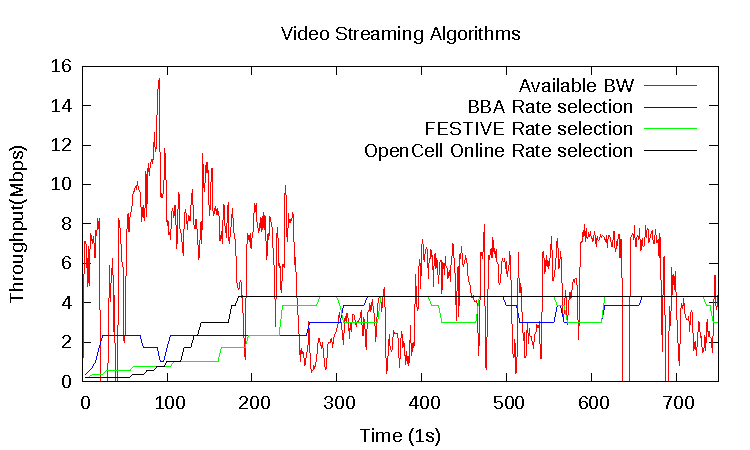
\includegraphics[width=\linewidth]{pictures/ATT.pdf}
 \caption{A sample trace from one major 4G network}
\end{figure}

\begin{table}[t]

\begin{tabular} {|c |c |c |c |}
\hline
\textbf{ Improvement} &\textbf{Quality} &\textbf{Stability} & \textbf{Interruption}\\ \hline
BBA(3G)  & 1.16x& 2.87x& 1x \\ \hline
FESTIVE(3G)    & 1.39x & \textcolor{red}{0.68x}&2.5x\\ \hline
BBA(4G) & 1.15x&3.8x& 1x* \\ \hline
FESTIVE(4G) & 1.32x& 3.6x& 1x* \\ \hline
\end{tabular}
\centering
\caption{\large Improvement with oracle estimator\newline \small*no interruption occurred during play} \label{cap:table}
\end{table}



\subsection{Oracle Estimator}\label{sub:oracle}
In this section, the algorithm is using an "oracle" estimator, to show the space of improvement.

\emph{Key metrics improvement:} we measure three different metrics: quality (play efficiency), stability and interrupts. Our algorithm outperforms the other two algorithms in all traces in terms of all three metrics except for stability in two 3G trace comparing to FESTIVE, and the summary is in \autoref{cap:table}. For the traces where FESTIVE achieves higher stability, FESTIVE tends to stay at low play bit rates and thus has much lower quality and link utilization, we also note in these traces the stability issue is less important: our algorithm has 5.5 switches on average while FESTIVE has 3 switches, and in all other traces all algorithms have $>$6 switches. 
\begin{figure}[t]
\centering
 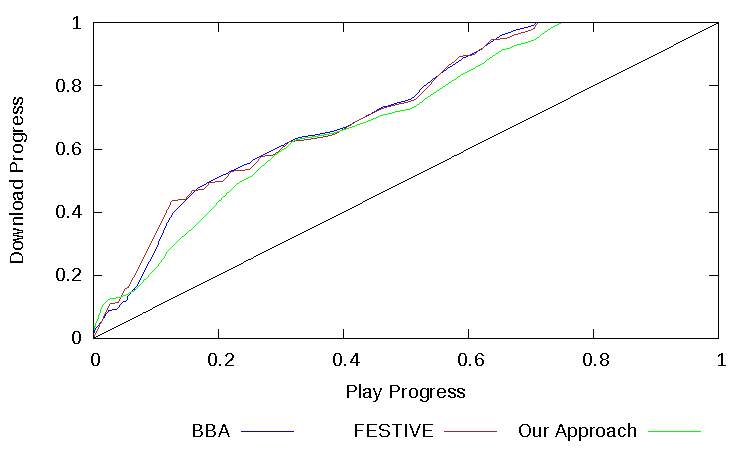
\includegraphics[width=\linewidth]{pictures/ATT_downloading.pdf}
 \caption{Buffer Prefetching} \label{fig:download}
\end{figure}
%\emph{Key metrics improvement:} we measure four different metrics: quality (play efficiency), stability and interrupts. Link utilization measures the total download vs available bandwidth, and the value is one if the link is constantly saturated. Play efficiency measures during the play session, the video downloaded and played vs available bandwidth, in the case without prefetched chunks, download utilization and play efficiency are equal. Stability measures the number of bit rate switches and interrupts measures the occurrence of interruption. Our algorithm outperforms the other two algorithms in all traces in terms of all four metrics, and the summary is in \autoref{cap:table}.

\emph{Prefetched buffer size}: we also compare the prefetched buffer size between BBA and our approach. FESTIVE is not client video buffer based solution and only adds randomized scheduling if it reaches a certain buffer level, we extend that buffer level to $z=240s$ download and see no difference in terms of FESTIVE's efficiency, stability or interruption, since FESTIVE only looks at past 20 chunks. Comparing BBA, we have reduced buffer size significantly by 10-40 seconds even though both maximum buffer sizes $z=240$. One sample trace is in \autoref{fig:download}: ideally the download progress and play progress are on the red line, however due to prefetching the download time is always ahead of play time, or the download line is always above the red line and the gap is the client play buffer size.

\begin{table}[t]
\small
\begin{tabular} {|c|c|c|c|}
\hline
 &\textbf{BBA} &\textbf{FESTIVE} &\textbf{Our Approach} \\ \hline
Ramp-up Time& 560s& 260s& 144s\\ \hline\hline
Link Loss(30s)& 1.05 Mbps& 1.05 Mbps& 4.3 Mbps\\ \hline
Link Loss(45s)& 1.05 Mbps& 1.05 Mbps&1.05 Mbps\\ \hline
Link Loss(60s)& 0.235 Mbps& 1.05 Mbps&1.05 Mbps\\ \hline
\end{tabular}
\centering
\caption{Ramp-up time and resilience to link outage} \label{cap:table2}
\end{table}

\emph{Fast ramp up and resilience to connection loss:} we use a synthetic trace to test the algorithms' properties. We set the bandwidth to static at 4.3 Mbps to test ramp-up time. We also add 30, 45 and 60 seconds connection outage after 100 seconds 4.3 Mbps bandwidth to test the resilience of the algorithm. All algorithm encounters zero interruption in all cases, our algorithm and FESTIVE's play bit rates are 4.3 Mbps at the moment, while BBA's is 1.75 Mbps. (Note the difference between play time and download time, FESTIVE takes 260s play time to get to 4.3 Mbps, but at 100s download time FESTIVE is downloading video chunk at bit rate 4.3 Mbps, the gap is due to prefetching) Algorithms suffer from dropping to a lower quality, and the new low quality values are summarized in \autoref{cap:table2}. This shows our algorithm has a good performance margin in both ramp-up time and resilience to link loss. 



\emph{Comparison with Theoretical Max Quality}: for a formulation in
\autoref{subsec:offline}, we use IBM CPLEX to solve the mixed integer problem.
We again replayed the 16 traces and the result shows that our approach can
achieve 84\% of the efficiency upper bound. For the formulation in
\autoref{subsec:offline} one 3G trace has no feasible solution, and the reason
is from the zero-interruption constraint, which also justifies the inevitability
of interruption occurred in online algorithms. 
\xin{Why not show the upper bound together with others in Table 3,4 and Figure
2,3?}
\kelvin{The upper bound does not include the stability and also does not consider fast startup, so the comparison is not apple to apple. I was prone to take out the so-called upper bound, but some tend to stick to it}

%\emph{Comparison with Modified FESTIVE}\Note{Not done yet!}: to show the performance gain is from both the novel algorithm and exposed extra KPIs, we also modified FESTIVE: we feed FESTIVE with a future bandwidth instead of using its harmonic mean estimation. 

\begin{comment}
\begin{table}[t]

\begin{tabular} {|c |c |c |c |}
\hline
 Improvement &Quality &Stability & Interruption\\ \hline
BBA(3G)  & 1.16x&1.6x &\textcolor{red}{0.9x} \\ \hline
FESTIVE(3G)& 1.40x &\textcolor{red}{0.86x}& 5x\\ \hline
BBA(4G) & 1.17x& 1.9x& N/A \\ \hline
FESTIVE(4G) & 1.14x& 3.4x& N/A \\ \hline
\end{tabular}
\centering
\caption{Improvement with noisy estimator} \label{cap:table2}
\end{table}
\end{comment}
\subsection{Noisy Estimator}\label{sub:noisy}
We use a synthetic estimator for prediction and show that when the prediction is
roughly accurate with a certain degree of error rate, our algorithm is robust to
achieve a close-to-optimal performance. We conduct a sensitive study for the new
algorithm with the noisy estimator. The synthetic estimator uses a noisy factor
with a distribution of Gauss(1,0.2) or Uniform(0.5, 1.5) when offering predicted
bandwidth. Through repetitive replay, we found the algorithm achieves about the
same performance in all traces, but with around 10\% chance we have significant
degradation in stability (1.5x quality switches) in the repetitive replay. 
\xin{Why cannot we predict with ARIMA?}


\section{Architecture} \label{sec:Architecture}
This section starts with the architecture of a scalable prediction system in
\autoref{subsec:prediction_system}, and then we discuss the feasibility and
advantages of inline method to expose KPIs in \autoref{subsec:exposingAPI}.
\subsection{Scalable Prediction System} \label{subsec:prediction_system} We
propose a two-tiered system to implement an KPI computing system. We have a
proxy sitting at data plane; and local and central bandwidth estimator at control
plane. The local bandwidth estimator communicates with eNodeBs and it takes
channel quality, number of active users, cell load and users' queue size etc.
information as inputs and compute the available bandwidth for each user. A local
bandwidth estimator is logically distributed in the RAN and thus can be easily
scale-out. Meanwhile the central bandwidth estimator sits in the core network
and it summarizes local BW estimation and MME Mobility information to compute
the final bandwidth prediction for a user. In most cases one local estimation is
enough, however in cases like handoff we need choose among several local
estimations. Central estimators can be
scale-out with MMEs. Our architecture is generic and able to integrate into both
3G and 4G networks. 

Once the computation work is finished, the central estimator sends the
information to the proxy. 
 
\begin{figure}[tb]\label{fig:Architecture}
 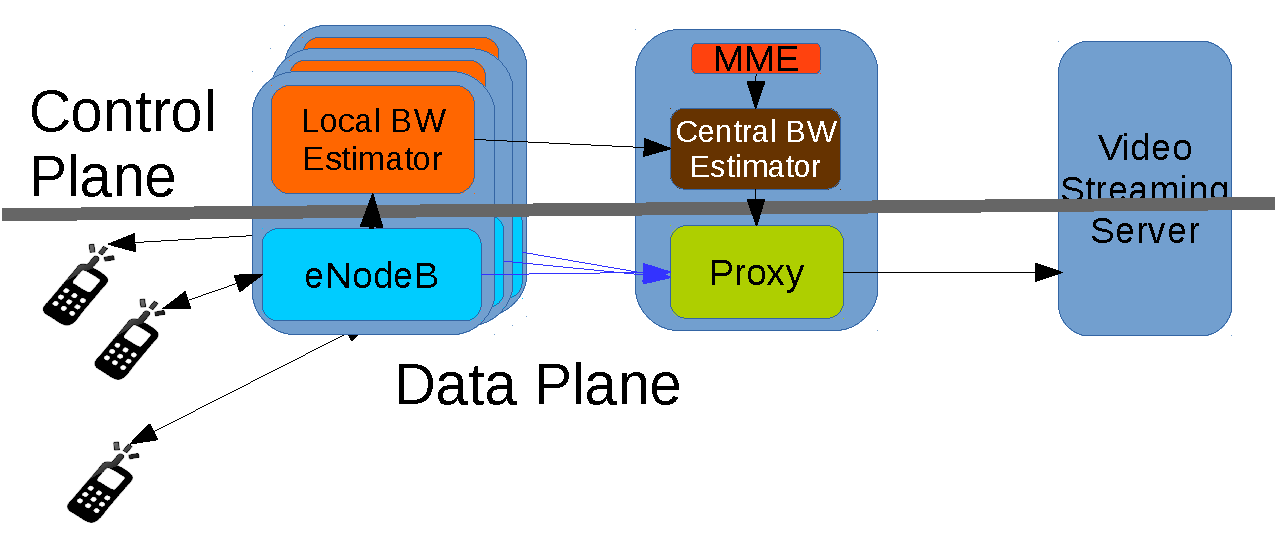
\includegraphics[width=\linewidth]{pictures/architecture2.pdf}
 \caption{Architecture for KPI Computing And Feedback}
\end{figure}


\subsection{KPI Exposure}\label{subsec:exposingAPI}
Current cellular networks already deploy proxies in the core network for
pacing purpose\cite{UntoldMiddleBoxStory}. It splits the TCP connection into two: server$\leftrightarrow
$proxy and proxy$\leftrightarrow $client. We can utilize the proxy for KPI
exposure. \emph{Sending to the server or the client?} We argue that exposing the
KPIs to the server causes less security concerns and network congestion. It also reduces the traffic in
the core network as sending to the client requires central estimator to send
back to local ones again. The downstream link carries majority of the traffic, upstream only has a small fraction of the traffic for feedback data. 
However since we let the server decide and the server in practice
may send back to the client's video play application. 

In terms of encoding the KPIs, there are several options: (i) in TCP; (ii) in
HTTP; and (iii) through a new connection. Inline methods have advantages over
new connection. First new connection method doubles the connections between the
server and the proxy. Second in practice CDNs are using public IPs, and the
video streaming connection and metric exposure connection may be directed to different private servers in CDN
load balancer. Inline methods both have some disadvantages. 
If we encode it into TCP option field, any middleboxes on the Internet may modify/drop the option field. 
The HTTP header may not be accessible since many streaming
services are using secure encrypted HTTP. Modifying HTTP header also requires DPI, which has a higher overhead than changing TCP.
\begin{figure}[t]\label{fig:Datagram}
 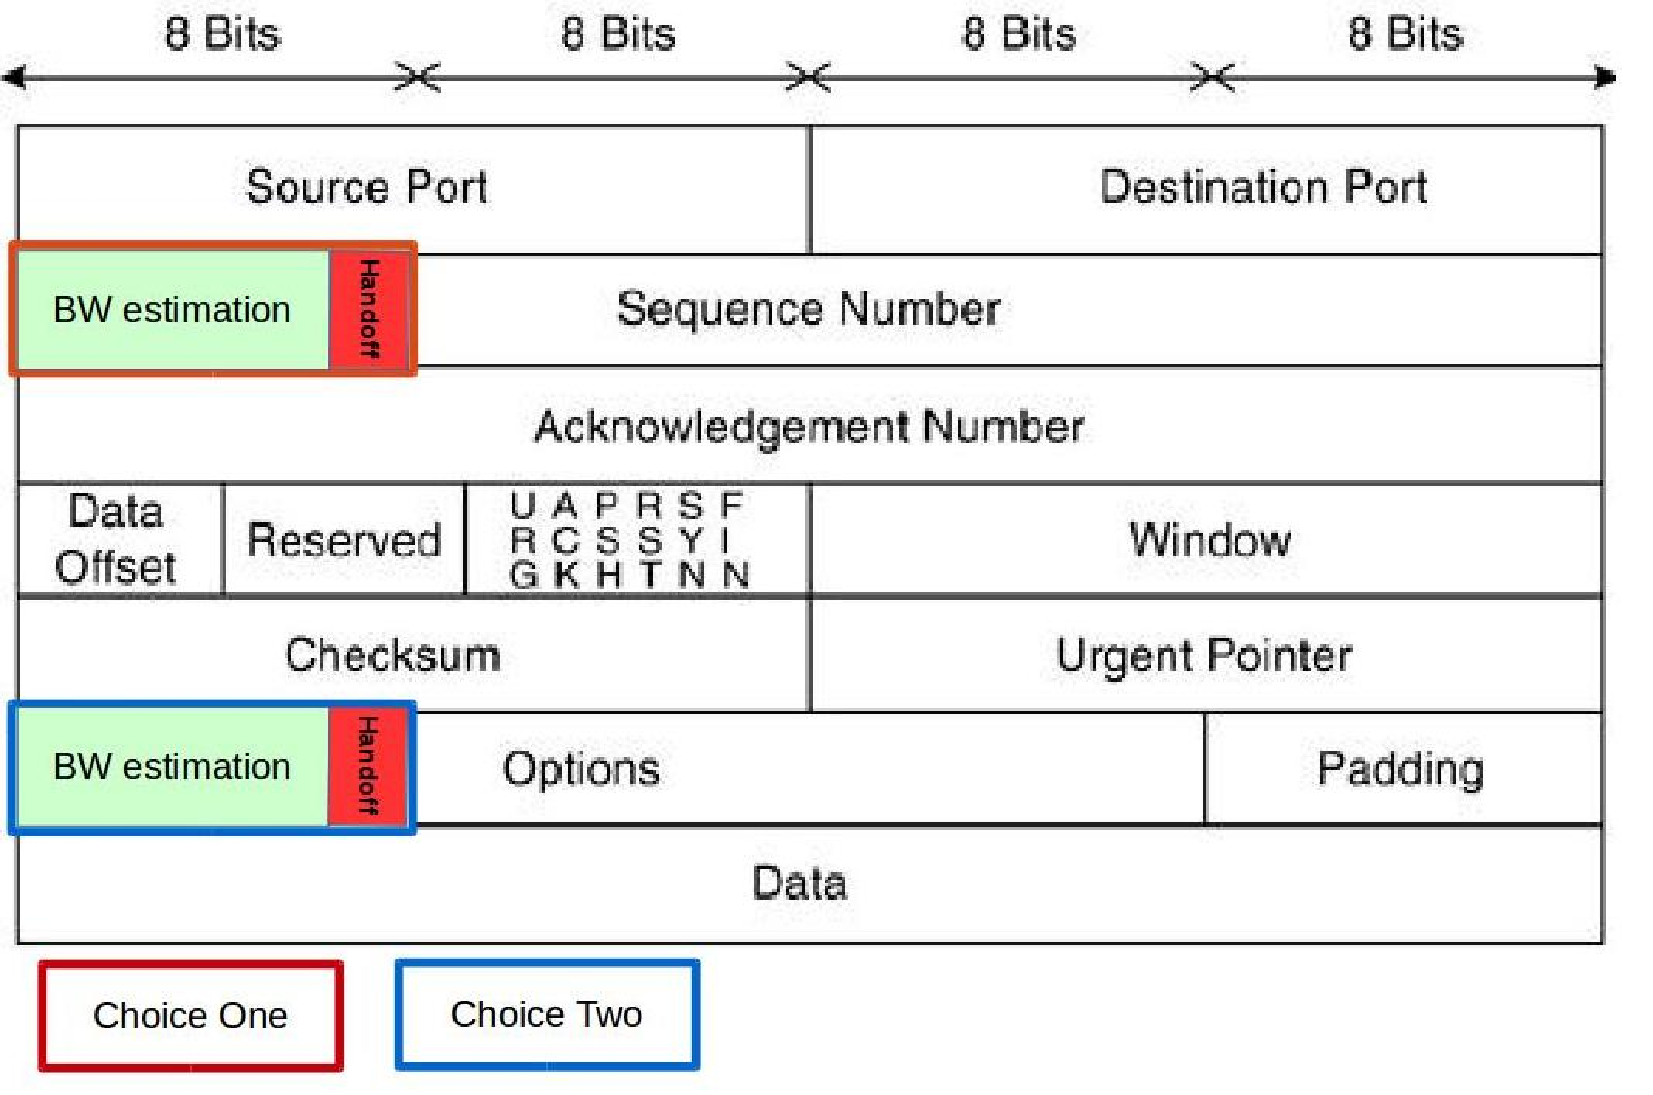
\includegraphics[width=\linewidth]{pictures/datagram.pdf}
 \caption{Datagram for exposing KPIs, it can be encoded in either option field or sequence number}
\end{figure}

One alternative approach is to encode in sequence number, if both content providers and cellular service providers are willing to collaborate. Since sequence number filed has 32 bits, we can reserve 8 bits for KPI exposure. In particular, we can use 7 bits for a floating number and 1 bit for handoff. Seven bits can be divided into integer and fractional parts, 3 bits for integer and 4 bits for fractional, it has a precision of 0.063 Mbps, or 63 Kbps and a maximum value of 8.94 Mbps, which is sufficient for today's video streaming bit rate selection where the range is between 0.2 to 4 Mbps.
At the same time it can still support 16 million packets before wrapping around. The bandwidth estimation is close to random so it holds the random feature of initial sequence number.

\xin{Would any middleboxes on the
Internet (between the proxy and the server) modify/drop the TCP option fields?}

\xin{Can we say a bit more about API here? What do the APIs look like? Give an
example and show how it is encoded in TCP option field.}

<emir>

In this section, we briefly describe the proposed architecture for realizing OpenCell concept. While alternative architectures are certainly possible, we aim for easy integration with the client-driven adaptation process in the state-of-the-art DASH systems. Hence, the exposed information or network state (e.g. predicted throughput) is made available to the client (video app), which can use it as a part of its adaptation logic, and/or share with the content server if desired.

The process of generating and exposing the information starts at the base station (eNodeB), where cell load, signal statistics and user throughput are collected. Based on collected data, predicted throughput is generated for all users and reported to the OpenCell server once per reporting interval. OpenCell server stores this information, which can be queried by user clients. Clients are typically HTTP-based and OpenCell server can use a simple HTTP-based API. Depending on requirements, clients can query the network state for the current or even past reporting periods. 

OpenCell servers can further process information received by base stations, e.g. to produce aggregated or long-term predictions. If base stations report every 500 ms, OpenCell servers may construct a prediction for 2, 5, or any number of seconds. This may depend on frequency the clients may query the OpenCell servers. 

In an application- or service-specific scenario, only certain apps or services are allowed to query OpenCell servers, enforcement of which is out of scope of this paper. However, it is possible to envision that all mobile clients could potentially have access. In a client-oriented architecture like ours, OpenCell servers are located inside the cellular core network and queried by video apps via HTTP. The prediction delivered by the OpenCell server will be valid for the next several seconds, typically on the order of video chunk duration. Each response may include information on how often clients may issue queries and for how long the returned prediction is valid.

We estimate that the proposed architecture can scale up to the requirements of today's video streaming services. 
(Add actual numbers)












\section{Conclusion}\label{sec:conclusion}

 
 
\bibliographystyle{acm}
{\small
\bibliography{references}} 

\end{document}
